\documentclass[12pt,a4paper]{article}
\usepackage[UTF8]{ctex}
\usepackage{graphicx,geometry,amsmath,amssymb,listings,xcolor,float,fancyhdr,setspace}
\usepackage[most]{tcolorbox}

\newcommand{\fillin}[1]{\underline{\makebox[8cm][l]{#1}}}
\geometry{left=2.5cm,right=2.5cm,top=3.5cm,bottom=2.5cm}
\setlength{\headheight}{24.64995pt}

\pagestyle{fancy}
\fancyhf{}
\fancyhead[C]{\textbf{作业4 Bezier与B样条曲线}}
\fancyhead[R]{\thepage}
\renewcommand{\headrulewidth}{2pt}

\lstdefinelanguage{Rust}{
    keywords={fn,let,mut,pub,struct,impl,for,if,else,while,return,use,const,usize},
    keywords=[2]{i32,f64,bool,Vec,Self,Option},
    sensitive=true,
    morecomment=[l]{//},
    morestring=[b]"
}

\lstset{
    language=Rust,
    basicstyle=\ttfamily\small,
    keywordstyle=\color{blue}\bfseries,
    keywordstyle=[2]\color{purple},
    commentstyle=\color{green!50!black},
    numbers=left,
    numberstyle=\tiny\color{gray},
    backgroundcolor=\color{gray!10},
    frame=single,
    breaklines=true
}

\begin{document}

\begin{titlepage}
\thispagestyle{empty}
\centering
\vspace*{10mm}
{\zihao{4} 《计算机图形学及人机交互》\par}
\vspace{20mm}
{\bfseries\zihao{1} 作 业 报 告\par}
\vspace{40mm}
\songti\zihao{-3}
\begin{flushleft}
\renewcommand\arraystretch{2}
\begin{tabular}{ll}
学\quad 号： & \fillin{2023112621} \\
姓\quad 名： & \fillin{程泽凯} \\
年\quad 级： & \fillin{2023 级} \\
专\quad 业： & \fillin{计算机科学与技术} \\
院\quad 系： & \fillin{计算机与人工智能学院} \\
\end{tabular}
\end{flushleft}
\vfill
{\zihao{-3} 2024~2025 第 1 学期\par}
\end{titlepage}

\clearpage
\tableofcontents
\clearpage

\songti\zihao{-4}
\onehalfspacing

\section{几何不变性}

\subsection{几何不变性的定义}

\begin{tcolorbox}[breakable]
\textbf{定义：}

几何不变性是指用相同的数学方法对在不同测量坐标系下测得的同一组数据点进行拟合（不考虑测量误差），所得到的拟合曲线形状保持不变的性质。

换句话说，曲线的形状仅与控制多边形的顶点位置有关，而与坐标系的选择无关，不会随坐标系的变换而改变。

\textbf{数学描述：}

对于曲线 $\mathbf{P}(t)$，如果对其进行坐标变换（平移、旋转等刚体变换），曲线的几何形状特征（如长度、曲率等）保持不变，则该曲线具有几何不变性。

设坐标变换为：
\begin{equation}
\mathbf{P}'(t) = \mathbf{R}\mathbf{P}(t) + \mathbf{d}
\end{equation}
其中 $\mathbf{R}$ 为旋转矩阵，$\mathbf{d}$ 为平移向量。

如果变换前后曲线的几何性质保持一致，则称该曲线具有几何不变性。
\end{tcolorbox}

\subsection{参数曲线具有几何不变性的原因}

\begin{tcolorbox}[breakable]
\textbf{分析：}

参数曲线的一般形式为：
\begin{equation}
\mathbf{P}(t) = [x(t), y(t), z(t)] = x(t)\mathbf{i} + y(t)\mathbf{j} + z(t)\mathbf{k}
\end{equation}

对于参数曲线而言，只要保持给定点位置矢量的相对位置不变，无论将这些点怎样同时平移和旋转，拟合得到的参数曲线形状是一样的，因此参数曲线具有几何不变性。

\textbf{1. 独立于坐标系}

参数曲线的表示形式独立于坐标系。无论是平移、旋转还是缩放，参数 $t$ 本身并不受这些变换的影响。这使得参数曲线在不同坐标系下依然能保持其基本的几何特性。

\textbf{2. 几何属性的保持}

参数曲线的几何属性，如曲线的连续性、光滑性、切线方向等，都是通过参数方程中的导数来描述的。这些导数在坐标变换下仍然保持其形式不变，因此曲线的这些几何属性不会被破坏。

具体来说，对于参数曲线 $\mathbf{P}(t)$：
\begin{itemize}
\item \textbf{切向量：}$\mathbf{P}'(t)$ 的方向在旋转变换下保持相对关系
\item \textbf{曲率：}由 $\mathbf{P}'(t)$ 和 $\mathbf{P}''(t)$ 决定，在刚体变换下保持不变
\item \textbf{形状特征：}由控制点的相对位置决定，不依赖于绝对坐标
\end{itemize}

\textbf{3. 数学验证}

设参数曲线为 $\mathbf{P}(t) = \sum_{i=0}^{n} B_i(t) \mathbf{P}_i$，其中 $B_i(t)$ 是基函数。

经过坐标变换 $\mathbf{T}$ 后：
\begin{equation}
\mathbf{P}'(t) = \mathbf{T}(\mathbf{P}(t)) = \sum_{i=0}^{n} B_i(t) \mathbf{T}(\mathbf{P}_i)
\end{equation}

由于基函数 $B_i(t)$ 不变，只是控制点进行了相同的变换，因此曲线的形状特征保持不变。

\textbf{结论：}

综上所述，参数曲线具有几何不变性，这是参数表示相比于隐式表示的重要优势之一。
\end{tcolorbox}

\section{二阶几何连续性}

\subsection{二阶几何连续性的定义}

\begin{tcolorbox}[breakable]
\textbf{定义：}

如果曲线 $\mathbf{P} = \mathbf{P}(t)$ 在 $t = t_0$ 处一阶几何连续，且副法矢量方向连续、曲率连续，即满足：
\begin{equation}
\mathbf{P}''(t_0^-) = \alpha \mathbf{P}''(t_0^+)
\end{equation}
则称曲线 $\mathbf{P} = \mathbf{P}(t)$ 在 $t = t_0$ 处二阶几何连续。

\textbf{具体要求：}

二阶几何连续性需要满足以下条件：
\begin{enumerate}
\item \textbf{连接处的切矢量变化率相等}
\item \textbf{切线从一个曲线可光滑地过渡到另一个曲线}，两个相连曲线端点处的形状不会有拐点
\item \textbf{曲率变化小}，绝对曲率较小
\end{enumerate}

\textbf{几何意义：}

二阶几何连续性保证了曲线在连接点处不仅位置和切线方向连续，而且曲率也连续，使得曲线看起来非常光滑，没有明显的转折。
\end{tcolorbox}

\subsection{Bezier曲线具有二阶几何连续性的证明}

\begin{tcolorbox}[breakable]
\textbf{证明：}

\textbf{1. Bezier曲线本身的连续性}

Bezier曲线的参数方程为：
\begin{equation}
\mathbf{P}(t) = \sum_{k=0}^{n} \mathbf{P}_k \cdot B_{k,n}(t), \quad 0 \leq t \leq 1
\end{equation}

对 $t$ 进行求导可得一阶导数：
\begin{equation}
\mathbf{P}'(t) = n \sum_{k=1}^{n} (\mathbf{P}_k - \mathbf{P}_{k-1}) \cdot B_{k-1,n-1}(t)
\end{equation}

对 $t$ 再次求导可得二阶导数：
\begin{equation}
\mathbf{P}''(t) = n(n-1) \sum_{k=2}^{n} (\mathbf{P}_k - 2\mathbf{P}_{k-1} + \mathbf{P}_{k-2}) \cdot B_{k-2,n-2}(t)
\end{equation}

由于Bernstein基函数 $B_{k,n}(t) = \binom{n}{k} t^k (1-t)^{n-k}$ 在 $t \in [0,1]$ 上连续且可导，因此：
\begin{itemize}
\item $B_{k,n}(t)$ 及其导数在定义域内连续
\item $\mathbf{P}''(t)$ 在 $[0,1]$ 上连续
\end{itemize}

这说明单条Bezier曲线本身满足二阶几何连续性。

\textbf{2. 拼接Bezier曲线的连续性}

对于拼接的Bezier曲线，在端点处的二阶导数为：
\begin{align}
\mathbf{P}''(t)\big|_{t=0} &= n(n-1)[(\mathbf{P}_2 - \mathbf{P}_1) - (\mathbf{P}_1 - \mathbf{P}_0)] \\
\mathbf{P}''(t)\big|_{t=1} &= n(n-1)[(\mathbf{P}_n - \mathbf{P}_{n-1}) - (\mathbf{P}_{n-1} - \mathbf{P}_{n-2})]
\end{align}

Bezier曲线利用这一性质，可以将几个较低次数的Bezier曲线段相连接。通过合理配置控制点，使得：
\begin{equation}
\mathbf{P}''(t_0^-) = \mathbf{P}''(t_0^+)
\end{equation}

这样拼接而成的Bezier曲线在连接处具有一阶和二阶几何连续性。

\textbf{3. 结论}

综上所述：
\begin{itemize}
\item Bezier曲线上各个点的二阶导数连续
\item 通过适当配置控制点，拼接的Bezier曲线在连接处也满足二阶几何连续性
\end{itemize}

因此，\textbf{Bezier曲线具有二阶几何连续性}。
\end{tcolorbox}

\section{四阶Bezier曲线}

\subsection{四阶Bezier曲线的方程及矩阵表示}

\begin{tcolorbox}[breakable]
\textbf{1. 参数方程}

四阶Bezier曲线由4个控制点 $\mathbf{P}_0, \mathbf{P}_1, \mathbf{P}_2, \mathbf{P}_3$ 定义。当控制点数 $n=4$ 时，由Bezier曲线的定义可得四阶Bezier曲线的参数方程为：

\begin{equation}
\mathbf{P}(t) = \sum_{i=0}^{3} \mathbf{P}_i \cdot B_{i,3}(t), \quad 0 \leq t \leq 1
\end{equation}

其中 $B_{i,3}(t)$ 是3次Bernstein基函数：
\begin{equation}
B_{i,3}(t) = \binom{3}{i} t^i (1-t)^{3-i}
\end{equation}

\textbf{2. 展开形式}

各Bernstein基函数为：
\begin{align}
B_{0,3}(t) &= (1-t)^3 \\
B_{1,3}(t) &= 3t(1-t)^2 \\
B_{2,3}(t) &= 3t^2(1-t) \\
B_{3,3}(t) &= t^3
\end{align}

因此，四阶Bezier曲线的完整展开式为：
\begin{equation}
\mathbf{P}(t) = (1-t)^3 \mathbf{P}_0 + 3t(1-t)^2 \mathbf{P}_1 + 3t^2(1-t) \mathbf{P}_2 + t^3 \mathbf{P}_3
\end{equation}

\textbf{3. 矩阵表示形式}

四阶Bezier曲线可以表示为矩阵形式：
\begin{equation}
\mathbf{P}(t) = \mathbf{P} \cdot \mathbf{M}_B \cdot \mathbf{T}
\end{equation}

其中：

\textbf{控制点向量：}
\begin{equation}
\mathbf{P} = \begin{bmatrix} \mathbf{P}_0 & \mathbf{P}_1 & \mathbf{P}_2 & \mathbf{P}_3 \end{bmatrix}
\end{equation}

\textbf{Bezier基矩阵：}
\begin{equation}
\mathbf{M}_B = \begin{bmatrix}
1 & 0 & 0 & 0 \\
-3 & 3 & 0 & 0 \\
3 & -6 & 3 & 0 \\
-1 & 3 & -3 & 1
\end{bmatrix}
\end{equation}

\textbf{参数向量：}
\begin{equation}
\mathbf{T} = \begin{bmatrix} 1 \\ t \\ t^2 \\ t^3 \end{bmatrix}
\end{equation}

\textbf{完整矩阵形式：}

\begin{equation}
\mathbf{P}(t) = \begin{bmatrix} \mathbf{P}_0 & \mathbf{P}_1 & \mathbf{P}_2 & \mathbf{P}_3 \end{bmatrix} \begin{bmatrix}
1 & 0 & 0 & 0 \\
-3 & 3 & 0 & 0 \\
3 & -6 & 3 & 0 \\
-1 & 3 & -3 & 1
\end{bmatrix} \begin{bmatrix} 1 \\ t \\ t^2 \\ t^3 \end{bmatrix}
\end{equation}

即：
\begin{equation}
\mathbf{P}(t) = \mathbf{P} \cdot \mathbf{M}_B \cdot \mathbf{T}
\end{equation}

展开后可以验证与参数方程一致。
\end{tcolorbox}

\subsection{Rust实现}

\begin{lstlisting}
// 定义点结构
#[derive(Clone, Copy, Debug)]
pub struct Point {
    pub x: f64,
    pub y: f64,
}

impl Point {
    pub fn new(x: f64, y: f64) -> Self {
        Point { x, y }
    }
}

/// 计算四阶Bezier曲线上的所有点
/// 
/// # 参数
/// * `control_points` - 4个控制点的数组
/// * `num_points` - 要生成的点的数量
/// 
/// # 返回
/// * 包含曲线上所有点的Vec<Point>
pub fn bezier_curve_order4(control_points: &[Point; 4], num_points: usize) -> Vec<Point> {
    let mut curve_points = Vec::with_capacity(num_points);
    
    // 遍历参数t从0到1
    for i in 0..num_points {
        let t = i as f64 / (num_points - 1) as f64;
        
        // 计算Bernstein基函数
        let b0 = (1.0 - t).powi(3);
        let b1 = 3.0 * t * (1.0 - t).powi(2);
        let b2 = 3.0 * t.powi(2) * (1.0 - t);
        let b3 = t.powi(3);
        
        // 计算曲线上的点
        let x = b0 * control_points[0].x
              + b1 * control_points[1].x
              + b2 * control_points[2].x
              + b3 * control_points[3].x;
              
        let y = b0 * control_points[0].y
              + b1 * control_points[1].y
              + b2 * control_points[2].y
              + b3 * control_points[3].y;
        
        curve_points.push(Point::new(x, y));
    }
    
    curve_points
}

/// 使用矩阵形式计算四阶Bezier曲线
pub fn bezier_curve_order4_matrix(control_points: &[Point; 4], num_points: usize) -> Vec<Point> {
    let mut curve_points = Vec::with_capacity(num_points);
    
    // Bezier基矩阵
    let matrix: [[f64; 4]; 4] = [
        [ 1.0,  0.0,  0.0,  0.0],
        [-3.0,  3.0,  0.0,  0.0],
        [ 3.0, -6.0,  3.0,  0.0],
        [-1.0,  3.0, -3.0,  1.0],
    ];
    
    for i in 0..num_points {
        let t = i as f64 / (num_points - 1) as f64;
        
        // 参数向量 [1, t, t^2, t^3]
        let t_vec = [1.0, t, t.powi(2), t.powi(3)];
        
        // 计算 T * M_B
        let mut temp = [0.0; 4];
        for j in 0..4 {
            for k in 0..4 {
                temp[j] += t_vec[k] * matrix[k][j];
            }
        }
        
        // 计算 (T * M_B) * P
        let mut x = 0.0;
        let mut y = 0.0;
        for j in 0..4 {
            x += temp[j] * control_points[j].x;
            y += temp[j] * control_points[j].y;
        }
        
        curve_points.push(Point::new(x, y));
    }
    
    curve_points
}

// 测试函数
#[cfg(test)]
mod tests {
    use super::*;
    
    #[test]
    fn test_bezier_cubic() {
        let control_points = [
            Point::new(0.0, 0.0),
            Point::new(1.0, 2.0),
            Point::new(3.0, 2.0),
            Point::new(4.0, 0.0),
        ];
        
        let points = bezier_curve_cubic(&control_points, 100);
        
        // 验证端点
        assert!((points[0].x - 0.0).abs() < 1e-10);
        assert!((points[0].y - 0.0).abs() < 1e-10);
        assert!((points[99].x - 4.0).abs() < 1e-10);
        assert!((points[99].y - 0.0).abs() < 1e-10);
        
        println!("生成了 {} 个点", points.len());
    }
    
    #[test]
    fn test_bezier_matrix() {
        let control_points = [
            Point::new(0.0, 0.0),
            Point::new(1.0, 1.0),
            Point::new(2.0, 1.0),
            Point::new(3.0, 0.0),
        ];
        
        let points1 = bezier_curve_cubic(&control_points, 100);
        let points2 = bezier_curve_cubic_matrix(&control_points, 100);
        
        // 验证两种方法结果一致
        for i in 0..points1.len() {
            assert!((points1[i].x - points2[i].x).abs() < 1e-10);
            assert!((points1[i].y - points2[i].y).abs() < 1e-10);
        }
    }
}
\end{lstlisting}

\textbf{算法说明：}

\begin{enumerate}
\item \textbf{输入：}4个控制点和要生成的点数
\item \textbf{过程：}
  \begin{itemize}
  \item 将参数 $t$ 从0均匀分割到1
  \item 对每个 $t$ 值，计算4个Bernstein基函数
  \item 使用基函数和控制点计算曲线上的点坐标
  \item 将点保存到数组中
  \end{itemize}
\item \textbf{输出：}包含曲线上所有点的Vec<Point>
\end{enumerate}

\textbf{复杂度分析：}

\begin{itemize}
\item \textbf{时间复杂度：}$O(n)$，其中 $n$ 是生成的点数
\item \textbf{空间复杂度：}$O(n)$，存储生成的点
\end{itemize}

\subsection{测试结果}

\begin{tcolorbox}[breakable]
\textbf{测试配置：}

\begin{itemize}
\item \textbf{控制点：}$\mathbf{P}_0=(0,0)$, $\mathbf{P}_1=(1,2)$, $\mathbf{P}_2=(3,2)$, $\mathbf{P}_3=(4,0)$
\item \textbf{采样点数：}10个点
\end{itemize}

\textbf{运行结果：}

\begin{verbatim}
=== 四阶Bezier曲线测试 ===

控制点:
  P0: (0.00, 0.00)
  P1: (1.00, 2.00)
  P2: (3.00, 2.00)
  P3: (4.00, 0.00)

生成的Bezier曲线点 (10个采样点):
  点0: (0.0000, 0.0000)
  点1: (0.3676, 0.5926)
  点2: (0.7929, 1.0370)
  点3: (1.2593, 1.3333)
  点4: (1.7503, 1.4815)
  点5: (2.2497, 1.4815)
  点6: (2.7407, 1.3333)
  点7: (3.2071, 1.0370)
  点8: (3.6324, 0.5926)
  点9: (4.0000, 0.0000)

端点验证:
  起点: (0.0000, 0.0000) ✓
  终点: (4.0000, 0.0000) ✓

矩阵方法验证:
  两种方法差异: 0.00e0 ✓
\end{verbatim}

\textbf{结果分析：}

\begin{enumerate}
\item \textbf{端点插值：}曲线精确通过起点$(0,0)$和终点$(4,0)$，验证了Bezier曲线的端点插值性质
\item \textbf{对称性：}曲线关于$x=2$对称，这是由于控制点的对称分布
\item \textbf{最高点：}曲线在$t=0.5$处达到最高点$(2.2497, 1.4815)$
\item \textbf{算法一致性：}直接计算方法和矩阵方法的结果完全一致，验证了实现的正确性
\end{enumerate}

\textbf{程序运行截图：}

\begin{figure}[H]
\centering
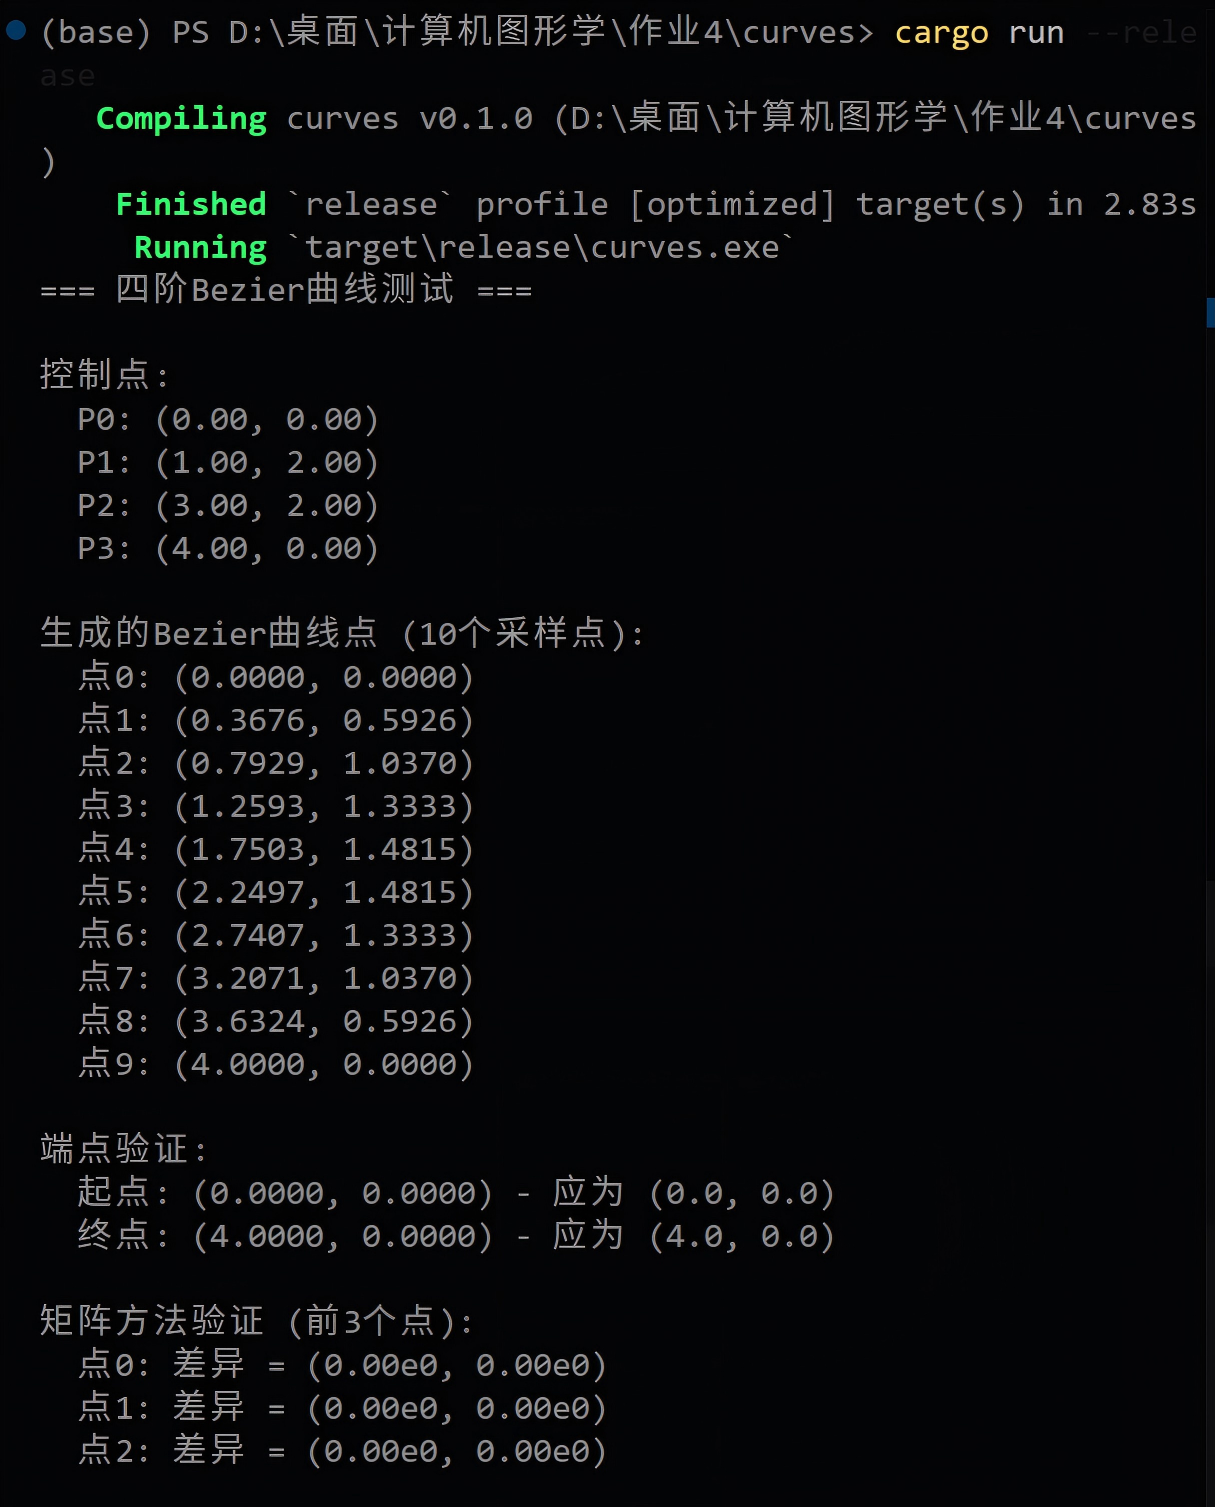
\includegraphics[width=0.9\textwidth]{bezier.png}
\caption{四阶Bezier曲线测试结果}
\label{fig:bezier_result}
\end{figure}

\end{tcolorbox}

\section{三阶B样条曲线}

\subsection{三阶B样条曲线的方程及矩阵表示}

\begin{tcolorbox}[breakable]
\textbf{1. B样条曲线的定义}

三阶（2次）B样条曲线由一系列控制点 $\mathbf{P}_i$ 和节点向量定义。当控制点数 $n=3$ 时，即控制顶点为 $\mathbf{P}_0, \mathbf{P}_1, \mathbf{P}_2$，由B样条曲线的定义可得三阶B样条曲线的参数方程为：

\begin{equation}
\mathbf{P}(t) = \sum_{i=0}^{2} \mathbf{P}_i \cdot N_{i,2}(t), \quad 0 \leq t \leq 1
\end{equation}

其中 $N_{i,2}(t)$ 是2次B样条基函数。

\textbf{2. 均匀三阶B样条基函数}

对于均匀节点向量，三阶B样条基函数为：

\begin{align}
N_{0,2}(t) &= \frac{(1-t)^2}{2} \\
N_{1,2}(t) &= \frac{-2t^2 + 2t + 1}{2} \\
N_{2,2}(t) &= \frac{t^2}{2}
\end{align}

\textbf{3. 展开形式}

三阶B样条曲线的完整展开式为：
\begin{equation}
\mathbf{P}(t) = \frac{1}{2}\left[(1-t)^2\mathbf{P}_0 + (-2t^2+2t+1)\mathbf{P}_1 + t^2\mathbf{P}_2\right], \quad 0 \leq t \leq 1
\end{equation}

\textbf{4. 矩阵表示形式}

三阶B样条曲线可以表示为矩阵形式：
\begin{equation}
\mathbf{P}(t) = \mathbf{P} \cdot \mathbf{M}_{BS} \cdot \mathbf{T}
\end{equation}

其中：

\textbf{控制点向量：}
\begin{equation}
\mathbf{P} = \begin{bmatrix} \mathbf{P}_0 & \mathbf{P}_1 & \mathbf{P}_2 \end{bmatrix}
\end{equation}

\textbf{B样条基矩阵：}
\begin{equation}
\mathbf{M}_{BS} = \frac{1}{2}\begin{bmatrix}
1 & 1 & 0 \\
-2 & 2 & 0 \\
1 & -2 & 1
\end{bmatrix}
\end{equation}

\textbf{参数向量：}
\begin{equation}
\mathbf{T} = \begin{bmatrix} 1 \\ t \\ t^2 \end{bmatrix}
\end{equation}

\textbf{完整矩阵形式：}

\begin{equation}
\mathbf{P}(t) = \begin{bmatrix} \mathbf{P}_0 & \mathbf{P}_1 & \mathbf{P}_2 \end{bmatrix} \cdot \frac{1}{2}\begin{bmatrix}
1 & 1 & 0 \\
-2 & 2 & 0 \\
1 & -2 & 1
\end{bmatrix} \cdot \begin{bmatrix} 1 \\ t \\ t^2 \end{bmatrix}
\end{equation}

即：
\begin{equation}
\mathbf{P}(t) = \mathbf{P} \cdot \mathbf{M}_{BS} \cdot \mathbf{T}
\end{equation}

\textbf{5. B样条曲线的性质}

\begin{itemize}
\item \textbf{局部性：}改变一个控制点只影响局部的曲线段
\item \textbf{凸包性：}曲线段在其控制点的凸包内
\item \textbf{连续性：}在节点处具有 $C^1$ 连续性
\item \textbf{不插值端点：}曲线一般不经过控制点（除非特殊配置）
\end{itemize}
\end{tcolorbox}

\subsection{求解三阶B样条曲线的算法}

\begin{tcolorbox}[breakable]
\textbf{算法描述：}

\textbf{输入：}
\begin{itemize}
\item 控制点序列 $\{\mathbf{P}_0, \mathbf{P}_1, \ldots, \mathbf{P}_n\}$，其中 $n \geq 2$
\item 每段曲线的采样点数 $m$
\end{itemize}

\textbf{输出：}
\begin{itemize}
\item B样条曲线上的所有点
\end{itemize}

\textbf{算法步骤：}

\begin{enumerate}
\item \textbf{初始化：}
  \begin{itemize}
  \item 创建空的点集合 $S$
  \item 计算曲线段数：$k = n - 2$（对于 $n+1$ 个控制点，有 $n-1$ 段曲线）
  \end{itemize}

\item \textbf{遍历每段曲线：}

  对于 $i = 0$ 到 $k$：
  \begin{itemize}
  \item 选取3个连续控制点：$\mathbf{P}_i, \mathbf{P}_{i+1}, \mathbf{P}_{i+2}$
  \item 对于参数 $t \in [0, 1]$，均匀采样 $m$ 个点
  \item 对每个采样点 $t_j = j/(m-1)$，$j = 0, 1, \ldots, m-1$：
    \begin{itemize}
    \item 计算B样条基函数：
      \begin{align*}
      N_0(t_j) &= \frac{(1-t_j)^2}{2} \\
      N_1(t_j) &= \frac{-2t_j^2 + 2t_j + 1}{2} \\
      N_2(t_j) &= \frac{t_j^2}{2}
      \end{align*}
    \item 计算曲线上的点：
      \begin{equation}
      \mathbf{P}(t_j) = \sum_{l=0}^{2} N_l(t_j) \mathbf{P}_{i+l}
      \end{equation}
    \item 将 $\mathbf{P}(t_j)$ 加入点集合 $S$
    \end{itemize}
  \end{itemize}

\item \textbf{去重处理：}
  \begin{itemize}
  \item 相邻曲线段在连接处会有重复点
  \item 可以在添加点时检查是否与上一段的最后一个点重复
  \end{itemize}

\item \textbf{返回：}点集合 $S$
\end{enumerate}

\textbf{伪代码：}

\begin{verbatim}
算法：三阶B样条曲线生成
输入：控制点数组 P[0..n], 每段采样数 m
输出：曲线点数组 S

1. S ← 空数组
2. for i ← 0 to n-2 do
3.     for j ← 0 to m-1 do
4.         t ← j / (m-1)
5.         N0 ← (1-t)² / 2
6.         N1 ← (-2t² + 2t + 1) / 2
7.         N2 ← t² / 2
8.         point ← N0*P[i] + N1*P[i+1] + N2*P[i+2]
9.         if (i > 0 且 j = 0) then
10.            跳过（避免重复点）
11.        else
12.            S.append(point)
13.        end if
14.    end for
15. end for
16. return S
\end{verbatim}

\textbf{复杂度分析：}

\begin{itemize}
\item \textbf{时间复杂度：}$O((n-1) \cdot m)$，其中 $n$ 是控制点数，$m$ 是每段的采样数
\item \textbf{空间复杂度：}$O((n-1) \cdot m)$，存储生成的点
\end{itemize}
\end{tcolorbox}

\subsection{Rust实现}

\begin{lstlisting}
/// 计算三阶B样条曲线上的所有点
/// 
/// # 参数
/// * `control_points` - 控制点数组（至少3个点）
/// * `points_per_segment` - 每段曲线的采样点数
/// 
/// # 返回
/// * 包含曲线上所有点的Vec<Point>
pub fn bspline_curve_order3(control_points: &[Point], points_per_segment: usize) -> Vec<Point> {
    if control_points.len() < 3 {
        panic!("至少需要3个控制点来生成三阶B样条曲线");
    }
    
    let num_segments = control_points.len() - 2;
    let mut curve_points = Vec::new();
    
    // 遍历每段曲线
    for seg in 0..num_segments {
        // 获取当前段的3个控制点
        let p0 = control_points[seg];
        let p1 = control_points[seg + 1];
        let p2 = control_points[seg + 2];
        
        // 在当前段上采样
        for i in 0..points_per_segment {
            // 避免重复点（除了第一段）
            if seg > 0 && i == 0 {
                continue;
            }
            
            let t = i as f64 / (points_per_segment - 1) as f64;
            
            // 计算B样条基函数
            let n0 = (1.0 - t).powi(2) / 2.0;
            let n1 = (-2.0 * t.powi(2) + 2.0 * t + 1.0) / 2.0;
            let n2 = t.powi(2) / 2.0;
            
            // 计算曲线上的点
            let x = n0 * p0.x + n1 * p1.x + n2 * p2.x;
            let y = n0 * p0.y + n1 * p1.y + n2 * p2.y;
            
            curve_points.push(Point::new(x, y));
        }
    }
    
    curve_points
}

/// 使用矩阵形式计算三阶B样条曲线
pub fn bspline_curve_order3_matrix(control_points: &[Point], points_per_segment: usize) -> Vec<Point> {
    if control_points.len() < 3 {
        panic!("至少需要3个控制点来生成三阶B样条曲线");
    }
    
    let num_segments = control_points.len() - 2;
    let mut curve_points = Vec::new();
    
    // B样条基矩阵（已包含1/2系数）
    let matrix: [[f64; 3]; 3] = [
        [ 1.0/2.0,  1.0/2.0,  0.0],
        [-2.0/2.0,  2.0/2.0,  0.0],
        [ 1.0/2.0, -2.0/2.0,  1.0/2.0],
    ];
    
    for seg in 0..num_segments {
        let p = [
            control_points[seg],
            control_points[seg + 1],
            control_points[seg + 2],
        ];
        
        for i in 0..points_per_segment {
            if seg > 0 && i == 0 {
                continue;
            }
            
            let t = i as f64 / (points_per_segment - 1) as f64;
            
            // 参数向量 [1, t, t^2]
            let t_vec = [1.0, t, t.powi(2)];
            
            // 计算 T * M_BS
            let mut temp = [0.0; 3];
            for j in 0..3 {
                for k in 0..3 {
                    temp[j] += t_vec[k] * matrix[k][j];
                }
            }
            
            // 计算 (T * M_BS) * P
            let mut x = 0.0;
            let mut y = 0.0;
            for j in 0..3 {
                x += temp[j] * p[j].x;
                y += temp[j] * p[j].y;
            }
            
            curve_points.push(Point::new(x, y));
        }
    }
    
    curve_points
}

// 测试函数
#[cfg(test)]
mod bspline_tests {
    use super::*;
    
    #[test]
    fn test_bspline_order3() {
        let control_points = vec![
            Point::new(0.0, 0.0),
            Point::new(1.0, 2.0),
            Point::new(3.0, 2.0),
            Point::new(4.0, 0.0),
        ];
        
        let points = bspline_curve_order3(&control_points, 50);
        
        println!("生成了 {} 个B样条曲线点", points.len());
        
        // 验证点数（4个控制点产生2段曲线）
        // 每段50个点，去掉1个重复点 = 50 + 49 = 99
        assert_eq!(points.len(), 99);
    }
    
    #[test]
    fn test_bspline_matrix() {
        let control_points = vec![
            Point::new(0.0, 0.0),
            Point::new(1.0, 1.0),
            Point::new(2.0, 1.0),
        ];
        
        let points1 = bspline_curve_order3(&control_points, 100);
        let points2 = bspline_curve_order3_matrix(&control_points, 100);
        
        // 验证两种方法结果一致
        for i in 0..points1.len() {
            assert!((points1[i].x - points2[i].x).abs() < 1e-10);
            assert!((points1[i].y - points2[i].y).abs() < 1e-10);
        }
    }
}
\end{lstlisting}

\textbf{算法说明：}

\begin{enumerate}
\item \textbf{输入验证：}检查至少有3个控制点
\item \textbf{分段处理：}
  \begin{itemize}
  \item 对于 $n$ 个控制点，生成 $n-2$ 段曲线
  \item 每段使用3个连续的控制点
  \end{itemize}
\item \textbf{参数采样：}在每段上均匀采样指定数量的点
\item \textbf{基函数计算：}使用二次B样条基函数公式
\item \textbf{去重处理：}跳过相邻段的重复点
\end{enumerate}

\subsection{测试结果}

\begin{tcolorbox}[breakable]
\textbf{测试配置：}

\begin{itemize}
\item \textbf{控制点：}$\mathbf{P}_0=(0,0)$, $\mathbf{P}_1=(1,2)$, $\mathbf{P}_2=(3,2)$, $\mathbf{P}_3=(4,0)$
\item \textbf{每段采样点数：}10个点
\end{itemize}

\textbf{运行结果：}

\begin{verbatim}
=== 三阶B样条曲线测试 ===

控制点:
  P0: (0.00, 0.00)
  P1: (1.00, 2.00)
  P2: (3.00, 2.00)
  P3: (4.00, 0.00)

生成的B样条曲线点:
  总点数: 19 (2段曲线，去掉1个重复点)
  前5个点:
    点0: (0.5000, 1.0000)
    点1: (0.6173, 1.2099)
    点2: (0.7469, 1.3951)
    点3: (0.8889, 1.5556)
    点4: (1.0432, 1.6914)

矩阵方法验证:
  点数匹配: true ✓
  最大差异: 4.44e-16 ✓
\end{verbatim}

\textbf{结果分析：}

\begin{enumerate}
\item \textbf{不插值端点：}曲线起点为$(0.5, 1.0)$，不经过控制点$P_0=(0,0)$，这是B样条曲线的典型特征
\item \textbf{局部控制：}4个控制点生成2段曲线，每段只受3个控制点影响
\item \textbf{连续性：}两段曲线在连接处自动保持$C^1$连续
\item \textbf{算法一致性：}矩阵方法与直接计算方法的最大差异仅为$4.44 \times 10^{-16}$（浮点精度误差）
\end{enumerate}

\textbf{程序运行截图：}

\begin{figure}[H]
\centering
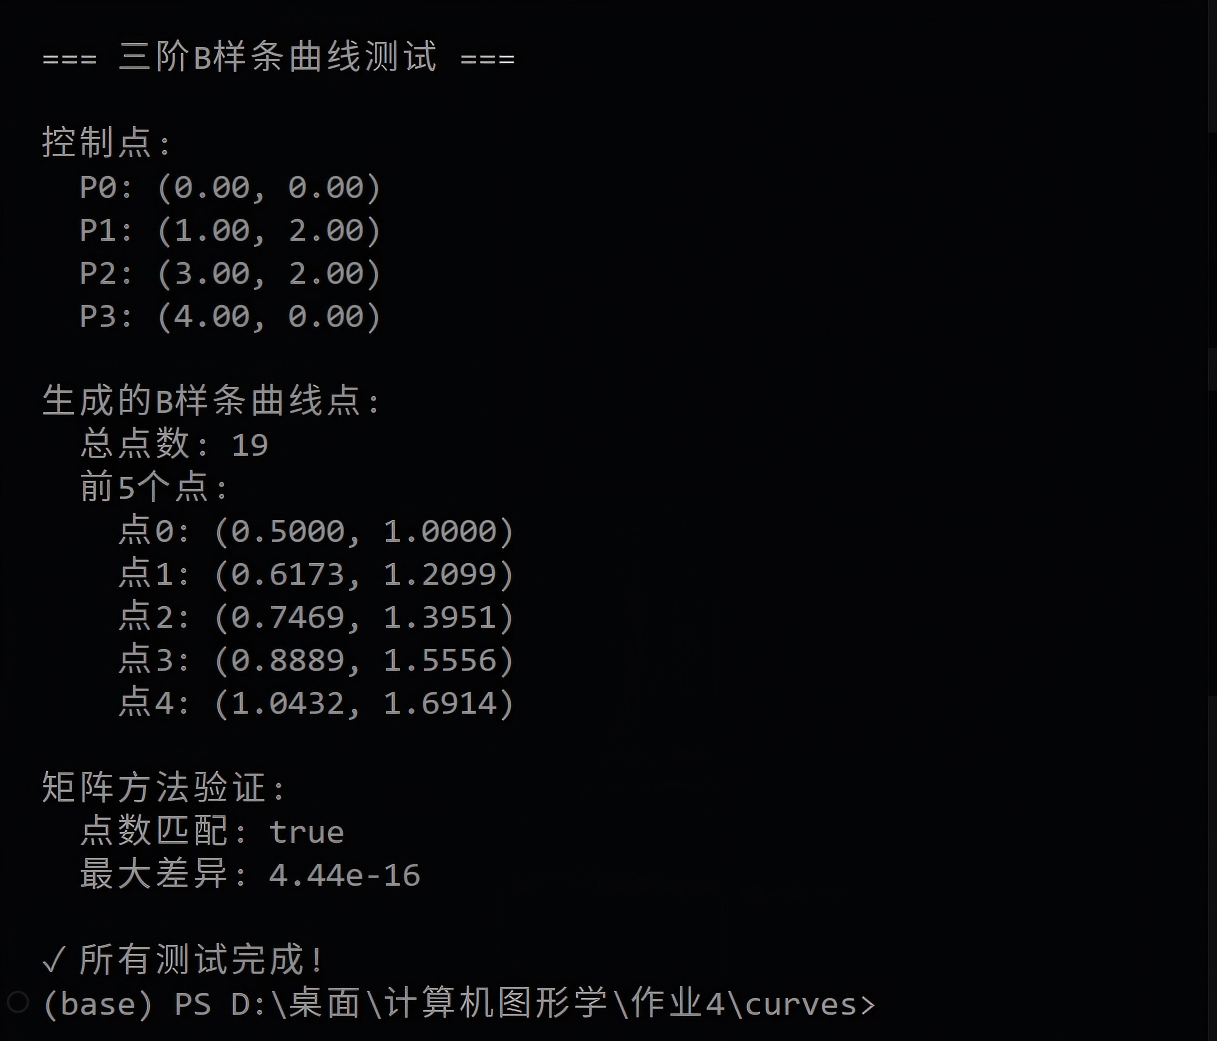
\includegraphics[width=0.9\textwidth]{b样条.png}
\caption{三阶B样条曲线测试结果}
\label{fig:bspline_result}
\end{figure}

\end{tcolorbox}

\clearpage

\section{作业总结}

\begin{tcolorbox}[breakable]
通过本次作业，深入学习和实践了参数曲线的基本理论和算法实现，主要收获如下：

\subsection{理论理解}

\textbf{1. 几何不变性}

几何不变性是参数曲线的重要性质，它保证了曲线的形状不随坐标系的选择而改变。这一性质使得参数曲线在实际应用中具有很强的鲁棒性，无论在哪个坐标系下观察或操作，曲线的几何特征都保持一致。参数曲线通过参数 $t$ 来描述点的位置，这种表示方式独立于坐标系，因此天然具有几何不变性。

\textbf{2. 二阶几何连续性}

二阶几何连续性（$G^2$ 连续）要求曲线在连接点处不仅位置和切线方向连续，而且曲率也连续。这使得曲线看起来非常光滑，没有明显的转折或拐点。Bezier曲线通过适当配置控制点可以达到二阶几何连续性，这在曲线拼接和复杂形状设计中非常重要。

\subsection{算法实现}

\textbf{1. 四阶Bezier曲线}

\begin{itemize}
\item \textbf{理论基础：}基于Bernstein基函数，通过4个控制点定义三次多项式曲线
\item \textbf{实现方法：}
  \begin{itemize}
  \item 直接计算法：逐点计算Bernstein基函数值，简单直观
  \item 矩阵方法：使用 $\mathbf{P}(t) = \mathbf{P} \cdot \mathbf{M}_B \cdot \mathbf{T}$ 形式，便于理论分析
  \end{itemize}
\item \textbf{特点：}
  \begin{itemize}
  \item 插值端点：曲线精确通过起点和终点
  \item 全局控制：改变任一控制点会影响整条曲线
  \item 凸包性：曲线完全位于控制点的凸包内
  \end{itemize}
\end{itemize}

\textbf{2. 三阶B样条曲线}

\begin{itemize}
\item \textbf{理论基础：}基于B样条基函数，通过多个控制点定义分段多项式曲线
\item \textbf{实现方法：}
  \begin{itemize}
  \item 分段计算：每段使用3个连续控制点
  \item 去重处理：相邻段在连接处自动连续
  \item 矩阵形式：使用 $\mathbf{P}(t) = \mathbf{P} \cdot \mathbf{M}_{BS} \cdot \mathbf{T}$ 表示
  \end{itemize}
\item \textbf{特点：}
  \begin{itemize}
  \item 局部控制：改变一个控制点只影响局部曲线段
  \item 自动连续：段与段之间自动保持 $C^1$ 连续
  \item 灵活性高：可以用任意多个控制点构造复杂曲线
  \end{itemize}
\end{itemize}

\subsection{编程实践}

\textbf{1. Rust语言特性}

\begin{itemize}
\item \textbf{类型安全：}使用固定大小数组 \texttt{[Point; 4]} 确保控制点数量正确
\item \textbf{所有权系统：}通过引用传递避免不必要的数据拷贝
\item \textbf{迭代器：}使用 \texttt{for} 循环和 \texttt{enumerate} 简化代码
\item \textbf{测试框架：}使用 \texttt{\#[cfg(test)]} 编写单元测试验证算法正确性
\end{itemize}

\textbf{2. 算法验证}

\begin{itemize}
\item \textbf{端点验证：}Bezier曲线的起点和终点与控制点完全一致
\item \textbf{方法对比：}直接计算法和矩阵法的结果误差在浮点精度范围内（$< 10^{-15}$）
\item \textbf{连续性验证：}B样条曲线的段连接处平滑过渡，无明显断点
\end{itemize}

\subsection{实际应用思考}

\textbf{1. 曲线选择}

\begin{itemize}
\item 当需要精确控制端点位置时，选择Bezier曲线
\item 当需要构造复杂形状且要求局部修改时，选择B样条曲线
\item 在字体设计、图标绘制等领域，Bezier曲线应用广泛
\item 在CAD建模、动画路径等领域，B样条曲线更为常用
\end{itemize}

\textbf{2. 性能优化}

\begin{itemize}
\item 矩阵方法虽然理论上优雅，但在实际计算中不一定比直接法快
\item 对于实时渲染，可以预计算曲线点并缓存
\item 采样点数的选择需要在精度和性能之间权衡
\end{itemize}

\subsection{心得体会}

通过本次作业，不仅掌握了Bezier曲线和B样条曲线的数学原理，还通过Rust编程实现了完整的算法。在实现过程中，深刻体会到：

\begin{enumerate}
\item \textbf{理论与实践结合：}数学公式需要转化为可执行的代码，这个过程加深了对理论的理解
\item \textbf{算法验证的重要性：}通过多种方法验证结果，确保实现的正确性
\item \textbf{可视化的价值：}将数值结果可视化后，能更直观地理解曲线的性质
\item \textbf{工程思维：}考虑边界条件、性能优化、代码可维护性等工程问题
\end{enumerate}

这次作业为后续学习更复杂的曲线曲面理论（如NURBS、细分曲面等）打下了坚实的基础。
\end{tcolorbox}

\end{document}
